\section{Experimental Evaluation}
\label{sec:eval}

\subsection{Experimental Setup}

We evaluate the proposed model on AnimeRun using the evaluation artifacts currently available in the repository. Following standard optical-flow practice, we report endpoint error (EPE) together with the fraction of pixels whose EPE is below $1$, $3$, and $5$ pixels. Lower EPE is better, while higher threshold accuracy is better. For the main comparison table, we only include methods for which the stored evaluation outputs expose the full threshold statistics required by this comparison. This avoids mixing fully evaluated runs with EPE-only summaries.

Our final reported model is the stabilized V5.1 object-memory dense system described in Section~\ref{sec:method}, followed by the low-learning-rate fine-tuning stage used in the final workspace `v5_1_object_memory_dense_parallel_ft`. The comparison is therefore aimed at a practical question: does adding dense recovery and the later stabilization recipe improve upon the earlier object-centric branch and strong dense or segmentation-aware baselines on AnimeRun?

\subsection{Quantitative Comparison}

\begin{table}[t]
\centering
\caption{AnimeRun comparison using methods whose stored artifacts include full EPE and threshold metrics. The reported V5.1 row corresponds to the best validation checkpoint from `v5_1_object_memory_dense_parallel_ft`.}
\label{tab:main_results}
\begin{tabular}{lcccc}
\hline
Method & EPE $\downarrow$ & 1px $\uparrow$ & 3px $\uparrow$ & 5px $\uparrow$ \\
\hline
MDFlow & 22.932 & 0.008 & 0.066 & 0.155 \\
UPFlow & 9.399 & 0.216 & 0.438 & 0.552 \\
V4 Hybrid SAM & 9.431 & 0.199 & 0.439 & 0.552 \\
V5 Object Memory & 10.028 & 0.155 & 0.414 & 0.534 \\
\hline
\textbf{V5.1 Object Memory Dense (Ours)} & \textbf{9.219} & \textbf{0.230} & \textbf{0.466} & \textbf{0.584} \\
\hline
\end{tabular}
\end{table}

Table~\ref{tab:main_results} shows that the final V5.1 system improves consistently over the earlier object-centric V5 baseline and over the stronger dense or segmentation-aware baselines for which full threshold outputs are available. Relative to the V5 object-memory baseline, V5.1 reduces EPE from $10.028$ to $9.219$ and improves the strict $1$px accuracy from $0.155$ to $0.230$. Relative to the strongest segmentation-aware baseline in the available comparison set, V4 Hybrid SAM, V5.1 improves EPE by approximately $0.212$ pixels while also improving all three threshold metrics. The gain over UPFlow is smaller in absolute EPE ($9.399 \rightarrow 9.219$), but the threshold accuracies still improve consistently.

At the same time, the results do not support an over-claim. The current V5.1 branch is clearly stronger than the earlier V5 object-only design, but it is still far from the originally desired sub-$7$ EPE regime. The remaining error is concentrated in large-displacement regions. At the best V5.1 checkpoint, the motion-stratified metrics are $3.036$ for $\mathrm{EPE}_{s<10}$, $19.160$ for $\mathrm{EPE}_{s10\text{-}50}$, and $90.547$ for $\mathrm{EPE}_{s>50}$. This pattern is important: most of the benchmark gain comes from small- and medium-motion regions, while the extreme-motion tail remains the main open problem.

For completeness, the repository also contains partial reference results that are not included in Table~\ref{tab:main_results}. The stored DDFlow artifact reports EPE $11.534$ with available $1$px and $3$px statistics but no stored $5$px metric, the stored UnFlow artifact reports only EPE $9.361$, and the older UnSAMFlow reproduction records best EPE $7.329$ in its training summary without matching threshold outputs. We therefore treat these as useful reference points, but do not mix them into the main threshold table.

\subsection{Model Analysis}

The internal comparison among design families is more revealing than the aggregate ranking alone. The V5 object-centric baseline preserves motion structure better than naive dense baselines in flat anime regions, but its affine object prior is too rigid to explain the local deformation that appears inside hair, clothing, and articulated limbs. This is exactly where V5.1 helps: the dense recovery stages improve local motion detail while the object-memory branch still supplies an explicit structural prior.

However, the detailed metrics also show what V5.1 has \emph{not} solved. The improvement over V4 Hybrid SAM and UPFlow is driven mainly by better performance in low- and medium-motion regions and by stronger strict threshold accuracy. In contrast, the large-motion tail changes only modestly. For example, $\mathrm{EPE}_{s>50}$ remains around $90.5$ for V5.1, close to the values of UPFlow and the strong V4 baselines. The current model therefore improves alignment and local sharpness without yet breaking the benchmark's hardest displacement regime.

\subsection{Qualitative Evaluation}

\begin{figure}[t]
\centering
\begin{minipage}[t]{0.49\linewidth}
    \centering
    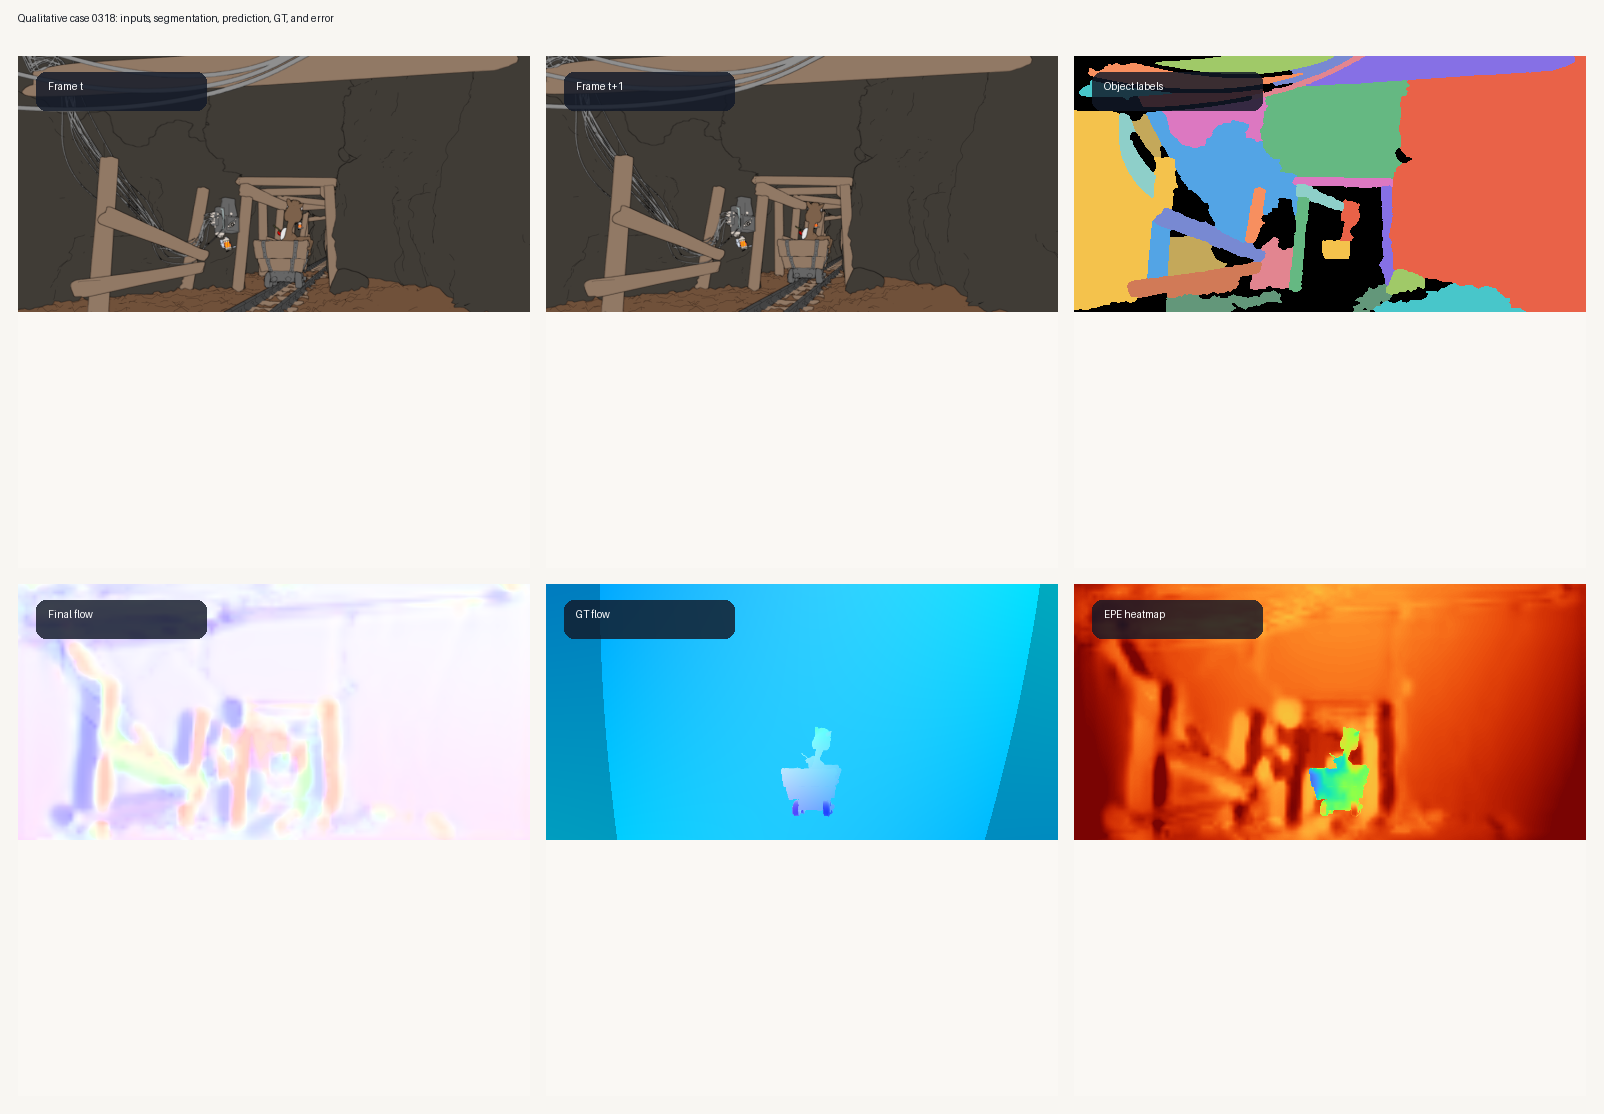
\includegraphics[width=\linewidth]{demo/v5_1_object_memory_dense_parallel_v4_paper/compact/eval_0318.png}
\end{minipage}\hfill
\begin{minipage}[t]{0.49\linewidth}
    \centering
    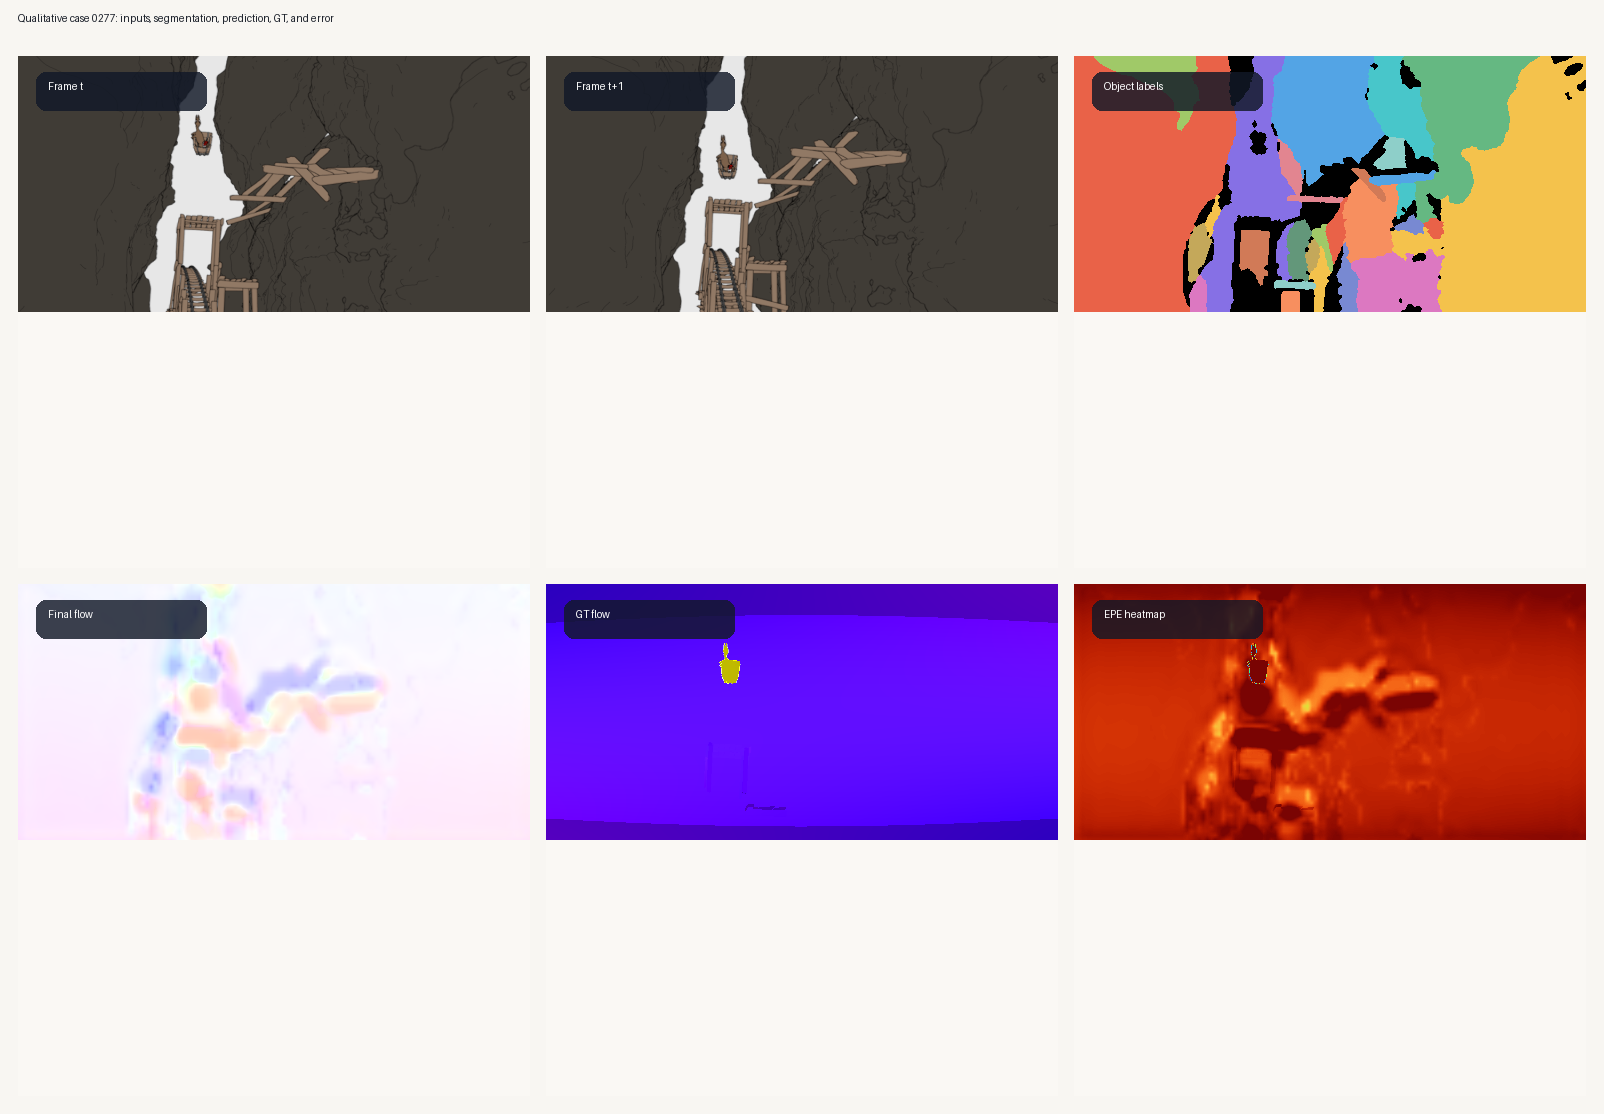
\includegraphics[width=\linewidth]{demo/v5_1_object_memory_dense_parallel_v4_paper/compact/eval_0277.png}
\end{minipage}
\caption{Qualitative evaluation on two AnimeRun clips. Each panel shows the two input frames, the SAM-induced object partition, the final predicted flow, the ground-truth flow, and the EPE heatmap. These examples are not ``easy'' low-error cases; instead, they show that the model often preserves the dominant object layout even when substantial residual error remains around thin boundaries and fast local motion.}
\label{fig:qualitative_eval_main}
\end{figure}

Figure~\ref{fig:qualitative_eval_main} illustrates behavior that the scalar metrics alone do not fully convey. In both examples, the predicted flow remains object-aligned and globally plausible, even though the absolute error is still noticeable. This is consistent with the quantitative picture: the model is usually structurally coherent, but still struggles to resolve the hardest local motion in the most difficult regions.

\begin{figure}[t]
\centering
\begin{minipage}[t]{0.49\linewidth}
    \centering
    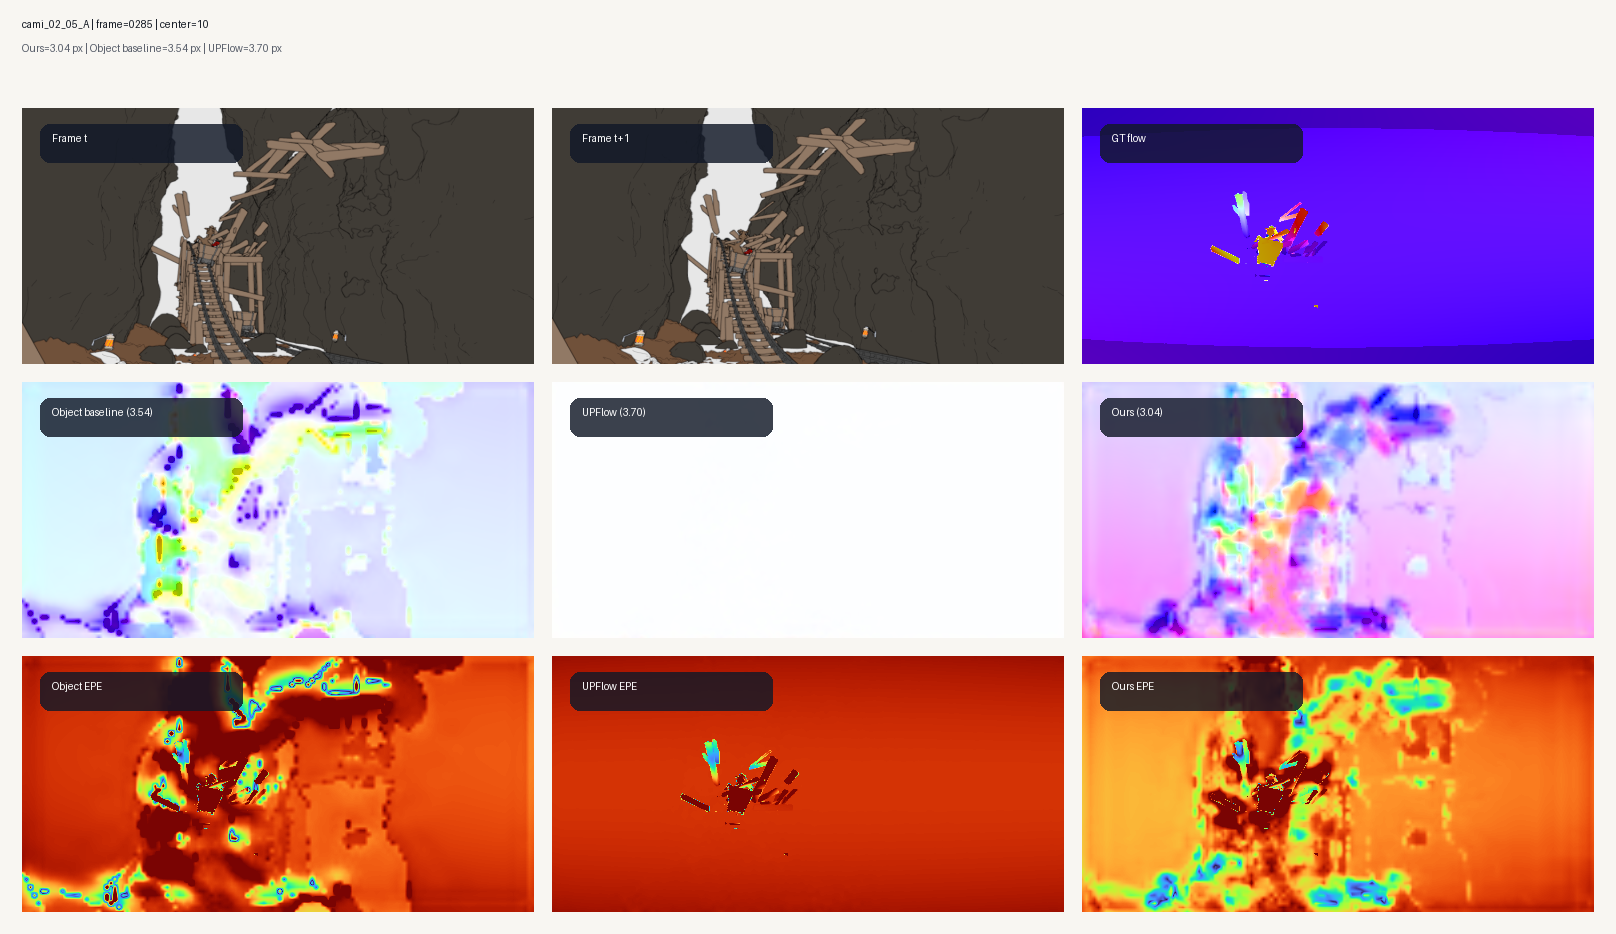
\includegraphics[width=\linewidth,height=0.42\textheight,keepaspectratio]{img/cami_02_05_A_compare_0285.png}
    
    \vspace{0.3em}
    \small Frame 0285
\end{minipage}\hfill
\begin{minipage}[t]{0.49\linewidth}
    \centering
    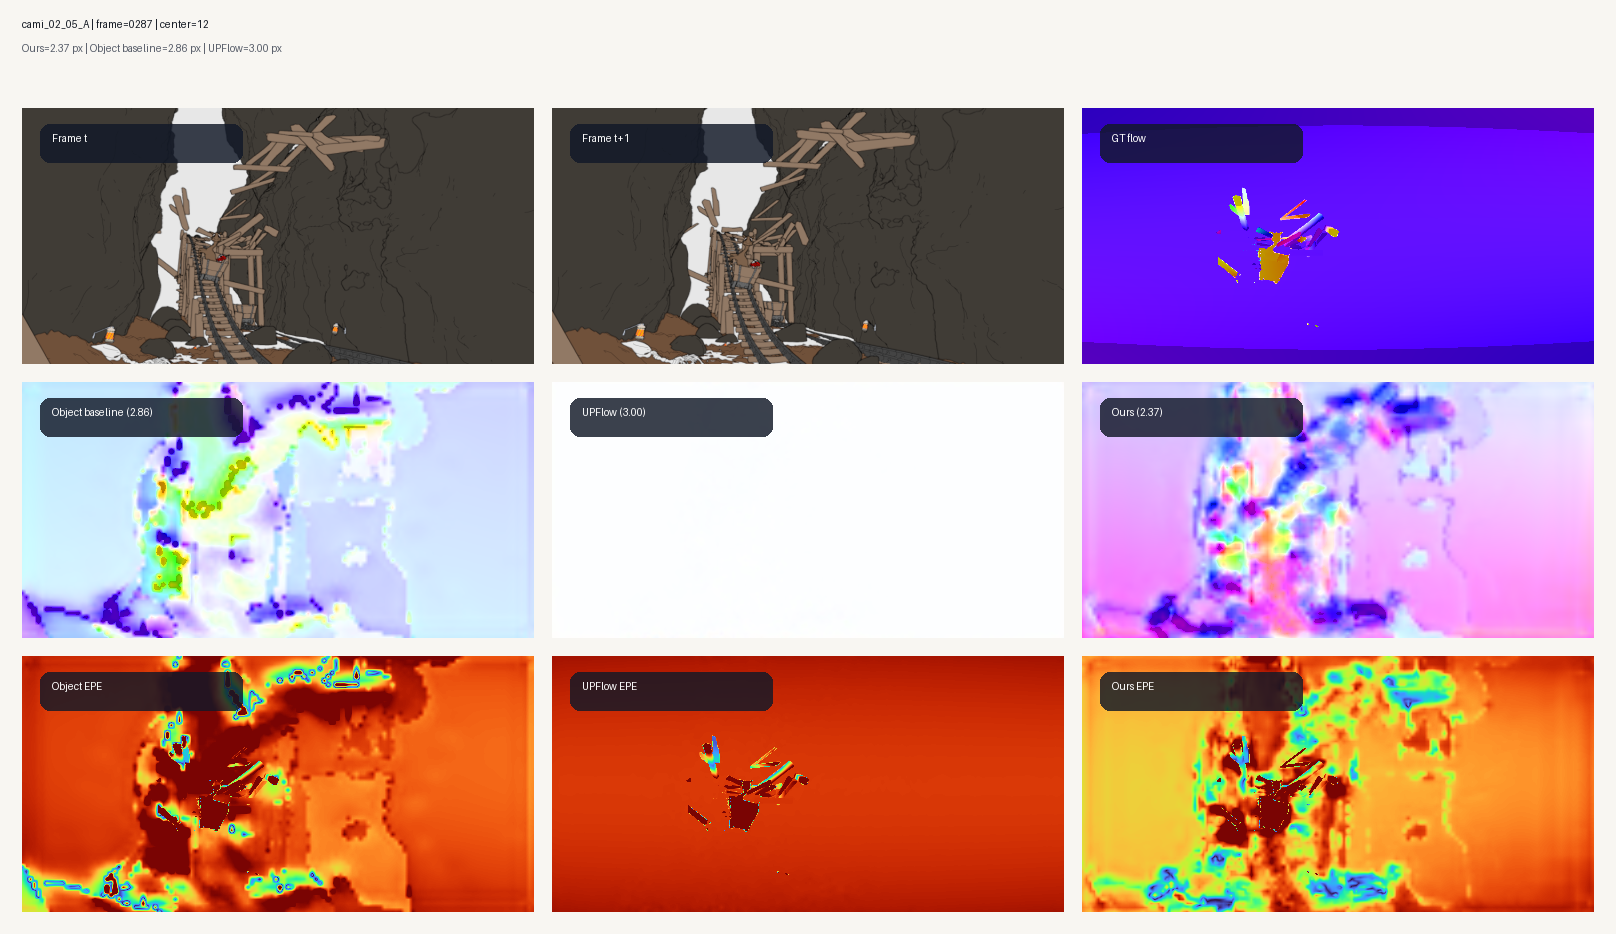
\includegraphics[width=\linewidth,height=0.42\textheight,keepaspectratio]{img/cami_02_05_A_compare_0287.png}
    
    \vspace{0.3em}
    \small Frame 0287
\end{minipage}
\caption{Targeted comparison against two weaker baselines: the object-centric V5 model without dense recovery and UPFlow. Each panel shows the two input frames, ground-truth flow, the three predicted flows, and the corresponding EPE heatmaps on a shared per-case color scale. For the selected frame 0285 example, V5.1 reduces mean EPE from $3.54$ and $3.70$ to $3.04$. For frame 0287, it reduces mean EPE from $2.86$ and $3.00$ to $2.37$. These examples support the intended role of dense recovery on top of object memory, but they should be read as targeted case studies rather than a substitute for the benchmark-wide table.}
\label{fig:qualitative_eval_vs_weaker}
\end{figure}

Figure~\ref{fig:qualitative_eval_vs_weaker} gives the clearest visual explanation of why V5.1 improves over the weaker object-only baseline. Relative to V5, the dense branch corrects the overly rigid affine prior inside the moving structure while preserving the broader object-aligned motion pattern. Relative to UPFlow, V5.1 avoids the weaker, more diffuse prediction that appears in the same regions. These examples are especially useful because they show the benefit of the hybrid design directly, not only as a scalar gain but as a concrete reduction in local motion error.

\begin{figure}[t]
\centering

\includegraphics[width=0.78\linewidth]{demo/v5_1_object_memory_dense_parallel_v4_paper/compact/eval_0306.png}
\caption{A harder close-up case with extremely large motion. The object partition remains coherent and the predicted flow still follows the dominant direction of motion, but the residual error grows substantially in the most extreme displacement region. This figure visualizes the same failure mode already suggested by the motion-stratified metrics.}
\label{fig:qualitative_eval_hard}
\end{figure}

The hard case in Figure~\ref{fig:qualitative_eval_hard} is important because it makes the remaining limitation explicit. The current model does not collapse under very large motion; it still preserves the object-level arrangement and broad motion direction. Yet this is also where the error grows most dramatically. Taken together, the qualitative section supports the same conclusion as the quantitative one: V5.1 is a meaningful improvement over the earlier object-centric branch and several practical baselines, but the large-displacement tail remains the dominant obstacle to substantially lower EPE.
